\documentclass[letterpaper, 10 pt, conference]{ieeeconf}  % Comment this line out if you need a4paper
\IEEEoverridecommandlockouts
\overrideIEEEmargins                                      % Needed to meet printer requirements.

%\usepackage{graphics} % for pdf, bitmapped graphics files
%\usepackage{epsfig} % for postscript graphics files
%\usepackage{mathptmx} % assumes new font selection scheme installed
%\usepackage{times} % assumes new font selection scheme installed
%\usepackage{amsmath} % assumes amsmath package installed
%\usepackage{amssymb}  % assumes amsmath package installed
%\usepackage{amsthm}
%\usepackage[style=ieee]{biblatex}
%\addbibresource{references.bib}
%
%%\theoremstyle{definition}
%%\newtheorem{definition}{Definition}[section]

%\usepackage{amssymb}
%\usepackage{graphicx}
%\usepackage{epstopdf}
%\usepackage{amsmath}
%\usepackage{subfigure}
%\usepackage{multirow}
%\usepackage{pbox}
%\usepackage{algorithm}
%\usepackage{algpseudocode}
%\usepackage{bm}
%\usepackage{url}


%%%%%%

%\documentclass[conference]{IEEEtran}
%
\usepackage{graphicx}
\usepackage{amsmath}
\usepackage{mathrsfs}
\usepackage{array}
\usepackage{enumerate}
\DeclareMathOperator*{\argmin}{arg\,min}
\DeclareMathOperator*{\argmax}{arg\,max}
\usepackage{amssymb}
\usepackage{mathtools}
\usepackage{breqn}
\usepackage{algorithm}
\usepackage{algorithmic}
\usepackage{varwidth}
%\usepackage[noend]{algpseudocode}
\makeatletter
\def\BState{\State\hskip-\ALG@thistlm}
\makeatother


\newcommand\NB[1]{$\spadesuit$\footnote{NB: #1}}
\newcommand\RP[1]{$\clubsuit$\footnote{RP: #1}}

\newcommand*{\Z}{\mathbb{Z}}
\newcommand*{\N}{\mathbb{N}}
% reference package for bibtex

%\usepackage{biblatex}
%\addbibresource{mybibliography.bib}

%\usepackage[
%backend=biber,
%style=numeric,
%sorting=ynt
%]{biblatex}

%\addbibresource{mybibliography.bib}


% correct bad hyphenation here
\hyphenation{op-tical net-works semi-conduc-tor}


\begin{document}
%
% paper title
% Titles are generally capitalized except for words such as a, an, and, as,
% at, but, by, for, in, nor, of, on, or, the, to and up, which are usually
% not capitalized unless they are the first or last word of the title.
% Linebreaks \\ can be used within to get better formatting as desired.
% Do not put math or special symbols in the title.
%\title{Using Hidden Markov Models to Improve Autonomous Vehicle Decision Making - Problem Formulation}
%\title{A Hidden Markov Models-based Approach for Automotive Predictive and Assistive Control}
\title{\LARGE \bf A Hidden Markov Model-based Approach for Predictive and Assistive Control in Semi-Autonomous Vehicles}
\author{Rahul Peddi and Nicola Bezzo%
\thanks{Rahul Peddi and Nicola Bezzo are with the Department of Systems and Information Engineering and the Charles L. Brown Department of Electrical and Computer Engineering, University of Virginia, Charlottesville, VA 22904, USA. Email: {\tt \{rp3cy, nb6be\}@virginia.edu}}
%\thanks{$^{2}$Esen Yel is with the Department of Systems and Information Engineering, University of Virginia, Charlottesville, VA 22904, USA. Email: {\tt ey3un@virginia.edu}}
}



%\author{\IEEEauthorblockN{Rahul Peddi$^1$ and Nicola Bezzo$^{1,2}$} 
%\IEEEauthorblockA{
%\small
%$^1$Department of Systems and Information Engineering\\
%\small
%$^2$Department of Electrical and Computer Engineering\\
%\small
%University of Virginia\\
%Email: \{rp3cy, nbezzo\}@virginia.edu}}
%\hyphenation{u-sing}


\maketitle

% As a general rule, do not put math, special symbols or citations
% in the abstract
\begin{abstract}
\end{abstract}

% no keywords




% For peer review papers, you can put extra information on the cover
% page as needed:
% \ifCLASSOPTIONpeerreview
% \begin{center} \bfseries EDICS Category: 3-BBND \end{center}
% \fi
%
% For peerreview papers, this IEEEtran command inserts a page break and
% creates the second title. It will be ignored for other modes.
\IEEEpeerreviewmaketitle



\section{Introduction}
% no \IEEEPARstart

%    Over the last few years, semi-autonomous and autonomous vehicles have become increasingly popular, but they have not replaced traditional vehicles entirely just yet. This leads to a hybrid environment; one that features vehicles of all levels of autonomy. Many of these vehicles to be equipped with some form of adaptive cruise control (ACC) or advance driver assistance systems (ADAS), both of which help the driver make safe decisions while operating the vehicle. These types of systems are forms of human-robot interaction. ACC performs actions autonomously and works at the command of a human who determines a target velocity and a safe following distance. ADAS, on the contrary, acts as an information system for human drivers. These systems, however, are limited in their capabilities as they require constant monitoring from the driver and are unable to predict if the driver will enter a dangerous situation in the future. In addition, these systems can fail to guarantee safety in rapidly transitioning environments.
    
    
%    Because these dangerous situations can occur so rapidly \NB{need citation here}, there is a need to increase the ability to guarantee safety when developing new systems \NB{what do you mean with new systems?} for human drivers. This can be done by increasing the ability to predict and adapt to what will happen in the future. A simple depiction of a danger situation is shown in Fig. \ref{fig:hiway}. \NB{figure needs improvements}

%\NB{I'll go back to this later...intro needs a lot of attention!}
 
%\NB{In a not far future, multiple vehicles with different level of autonomy will have to coexist and operate safely. Examples of such vehicles include cars, vessels, aerial vehicles. Different levels of autonomy are available 1 to 5 for cars, hobby  }   

%\NB{Semi-autonomous and autonomous vehicles are finding their way in our society rapidly. Although new advancements in sensing and autonomy are increasing safety by assisting drivers with line changing warning and assisted braking, } 
%\NB{here let's talk about the trolly problem and mention that we see humans as disturbance in this work! discuss about teleoperated robotics that is still big and assistive automation}

Semi-autonomous and autonomous vehicles are finding their way in our society rapidly. As these vehicles proliferate the roadways, we get a mixed environment, meaning that different levels of autonomy are available. Although new advancements in sensing and autonomy are increasing safety by assisting drivers with systems such as adaptive cruise control (ACC) \cite{acc} or advanced driver assistance systems (ADAS) \cite{adas}, these systems are far from perfect. ACC performs actions autonomously and works at the command of a human who determines a target velocity and a safe following distance. ADAS, on the other hand, acts as an information system for human drivers. These systems, however, are limited in their capabilities as they require constant monitoring from the driver and are unable to predict if the driver will enter a dangerous situation in the future. In addition, these systems can fail to guarantee safety in rapidly transitioning environments \cite{accfail}.
    

\begin{figure}[ht]
    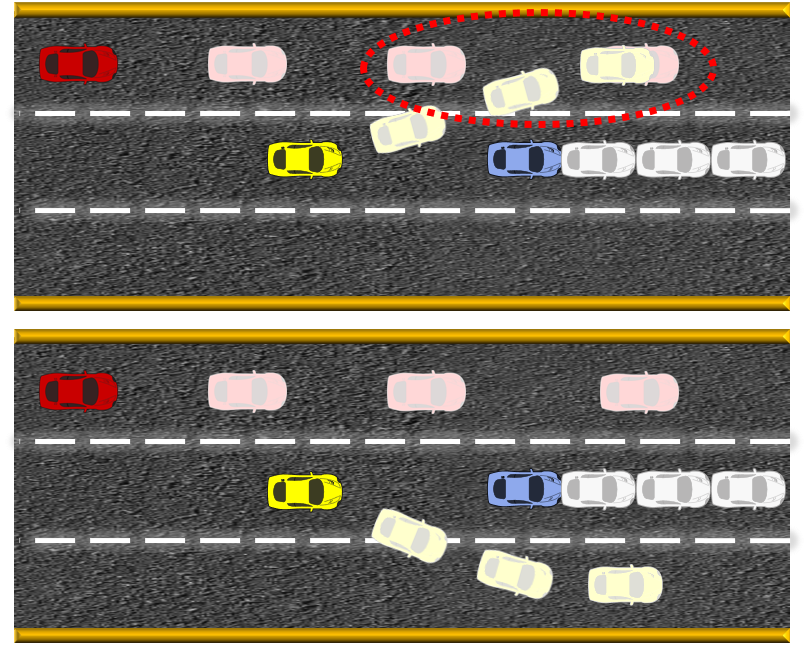
\includegraphics[width=0.48\textwidth]{highway.png}
    \caption{Two possible actions on a highway, where one leads to a dangerous situation in the future(top), and another minimizes risk (bottom)}
    \label{fig:hiway}
\end{figure}
    
    An example of such environment is a large multi-laned area with multiple vehicles. In Fig.\ref{fig:hiway}, a user is driving a vehicle (yellow car) behind a slower vehicle (blue car). In this case, both actions presented in Fig.\ref{fig:hiway} may appear safe to a driver at the moment, but as can be seen by the red circle, one of the lane changes is considerably riskier in the future, because a rapidly approaching vehicle (red car) will enter the same space as the user's vehicle. In this case, we see the driver's actions as potentially adversarial, or as a disturbance, and want to assist the driver. In order to prevent a riskier action from taking place, we are interested in predicting future states of other surrounding vehicles, assessing risk of collisions given the user's actions, and intervening and assisting the driver accordingly. This type of work can be approached as a type of Markov Chain, and we leverage Hidden Markov Model (HMM) theory as well, both of which are commonly used models for many cyber-physical systems (CPS).
    
     In this work, we aim to provide
    \begin{itemize}
    \item{a prediction method that can effectively and efficiently estimate the future positions of surrounding agents}
    \item{an adaptive framework that determines the adjustment of a user's actions and severity of such adjustment that should be made at any point in time}
    \end{itemize}
  
    
    The rest of this paper is organized as follows: in Section \ref{sec:relatedwork}, we discuss related work, and in Section \ref{sec:probform}, we formally define the problem. The general approach is discussed in Section \ref{sec:approach}. In Section \ref{sec:fmwk}, we discuss the specifics of the HMM-based framework, and how it is used to build models. We then use that framework to make online predictions in Section \ref{sec:ahmmpredupdate}, and show how we can fit the models to a system we are observing in Section \ref{sec:omf}. This is followed by a discussion of we use the framework, along with the predictions and fitting, to assist the user in Section \ref{sec:adapt}. Then we demonstrate our results with MATLAB simulations in Section \ref{sec:sims}. Lastly, we discuss our conclusions and future work in Section \ref{sec:concs}.

    
% You must have at least 2 lines in the paragraph with the drop letter
% (should never be an issue)

\section{Related Work} \label{sec:relatedwork}

The study of semi-autonomous and autonomous vehicles has been growing in recent years. As these options have become more available to the average consumer, driving environments have become more mixed, and researchers approach such environments from different viewpoints; those of improving the knowledge about the environment (i.e. prediction) and those that involve controlling for such environments (i.e. autonomy).

The authors in \cite{mpc} use velocity predictions derived from artificial neural networks and GPS systems for Model Predictive Control (MPC), which is presented as a highly complicated optimization problem, and the predictions are only evaluated for one vehicle at a time. The authors in \cite{velnn} and \cite{veldatadriv} take a data science approach and use large data-sets, along with very specific traffic information, in order to make predictions. The use of a Hidden Markov Model based approach for prediction is done in \cite{lanhmm}, where the authors develop an approach treating a vehicle as a hybrid state system to predict the trajectory of a certain behavior. This is done, while assuming knowledge of multiple In \cite{woohmm}, motivated by previous work in HMMs, the authors discuss using a simplified form of the hybrid state system with an HMM to improve lane change prediction scalability over multiple vehicles. In our work, we consider the problem of predicting future velocity and when lane changes are expected by leveraging the theories presented in \cite{mpc} and \cite{woohmm}. 

In terms of controlling vehicles in such environments, the authors in \cite{qmdp} use a Point-Based Markov Decision Process (QMDP) to estimate dangerous situations and react with the appropriate autonomous driving behavior in single-lane situations. The QMDP process employs a robust, but computationally intensive value iteration algorithm in order to do this. In \cite{predcost}, the authors present a prediction and cost-based (PCB) control strategy for autonomous vehicles given a known set of predicted scenarios. In this vein, \cite{vfh+} and \cite{vfh*} discuss reliable obstacle avoidance methods given that obstacle locations and characteristics are known based on artificial physics methods. In \cite{takeover}, with a human-factors based approach, the authors show multiple ways take-over requests can be generated in partially autonomous vehicles, including performance based and environment based characteristics. In our work, we leverage the idea of taking over from \cite{takeover}, along with the theories in \cite{vfh*} to control for future unsafe scenarios we detect in our predictions.

    
\section{Problem Formulation} \label{sec:probform}
 
In this work we are interested in finding an approach to proactively guarantee safety (i.e., something bad will never happen) in multi-vehicle systems. We focus on manned vehicles employing an hybrid autonomy scheme as defined in \cite{} in which the control authority is shared between the human and the on-board computer. For the sake of brevity we denote this class of vehicles as {\em hybrid autonomous vehicles} (HAVs), In our scheme, the on-board computer is used as a supervisory monitor to predict and assess safety and assist by correcting undesired human behaviors that may lead to unsafe situations and compromise the system's integrity. 

% control in which users may perform undesired actions that can compromise the safety of the entire system 
Formally the problem that we investigate in this work can be stated as: 

\textbf{Problem 1: \textit{Proactive Safe Assisted Planning and Control}:} 
      A hybrid autonomous vehicle (HAV) $h$ is moving in an environment in the presence of other vehicles $q \in R_h(t)$, where $R_h(t)$ is a time varying set of vehicles in sensing/communication range with $h$. The goal is to find a policy to:
    \begin{enumerate}
        \item  predict online other vehicles future states $s$ and their likelihood $p$. Formally, $\forall q \in R_h(t)$:
    \begin{equation}
   S_q=\{{s_q(t), s_q(t+1),..., s_q(t+T)}\}
       \end{equation}
       \begin{equation}
   P_q=\{{p_q(t), p_q(t+1),..., p_q(t+T)}\}
%     \forall q \in R_h(t), S_q=\{{s_q(t), s_q(t+1),..., s_q(t+T)}\}
    \end{equation}
     where $S_q$ is the set of all states, $s_q$, and $P$ is the set of all probabilities, $p_q$ over a finite time horizon $T\in\N$.  
%     assess their likelihood
%    \begin{equation}
%    P=\{{p_q(t), p_q(t+1),..., p_q(t+T)}\}
%    \end{equation}
%    where $P$ represents the set of all probabilities, $p_q(t)$ represents the probabilities at each time, $t$.
    \item assess the risk $0\leq r \leq1$ of a collision during $T$ and
    \item assist and intervene to correct the HAV actions to guarantee safety, i.e., obtain an input policy $U_h=\{{u_h(t), u_h(t+1),..., u_h(t+T)}\}$ such that the risk $r$ is always minimized. 
    \end{enumerate}
   In our specific multi-vehicle case, risk is a function of distance between vehicles. Hence minimizing risk is equivalent to guaranteeing the following:
    
%    surpasses a certain user defined level,$\rho$, we are able to minimize the risk, and guarantee,
    \begin{equation}
        ||{x_h(t)-x_q(t)}|| \geq d_{\textrm{min}}
    \end{equation}
     where $x_h(t)$ and $x_q(t)$ are the positions of the HAV and the $q^{\textrm{th}}$ surrounding vehicle at time $t$ and $d_{min}$ is a minimum safe distance.    
    
    It is important to note that the vehicle that we are assisting is primarily human operated, in the sense that we should intervene only when necessary. %\NB{we are not modifying anything, we are adapting and assisting its operation. This sentence needs to be rewritten.}.
    In other words, unless the user performs actions that we predict could lead to unsafe conditions, which we define as situations where $r_h>\rho$, where $\rho$ is a user defined threshold, we let the HAV perform his/her desired actions.

\section{Approach} \label{sec:approach}%\NB{We need to define this section in multiple sections: Offline/Online training; Online Prediction; Online Adaptation}
\begin{figure}[ht!]
    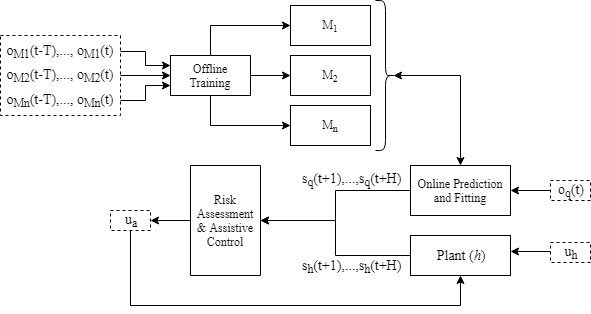
\includegraphics[width=0.48\textwidth]{approach.png}
    \caption{Block Diagram of the Approach}
    \label{fig:app}
\end{figure}
%\NB{figure is too blurry}
%\NB{that's not a pictorial representation, It's a block diagram.}
Our general approach, shown in Fig. \ref{fig:app} works to predict future states of other vehicles, $\{s_q(t+1),\ldots s_q(t+H)\}$ over time horizon $H$, thus inferring their behavior to better assess safety and intervene to avoid hazardous situations. We leverage a history of offline observations, $\{o(t-T),\ldots,o(t)\}$, to build different models, $\{M_1,\ldots,M_n\}$, that are used online to recognize and predict new vehicles' behaviors. Based on these predictions, we want to monitor whether our vehicle, $h$, could enter an unsafe state.
 based on the user input, $u_h$. 
 If such a unsafe action is detected, an autonomous control action, $u_a$, is deployed to assist and correct the user's intention. In the next sections, we will go over this framework, explaining in detail each block presented in Fig.~\ref{fig:app}.
 

%\NB{fix this}. %\NB{simplify}
 %\NB{this should go in the related work}.% In this work, we train multiple models offline over a horizon $T$, with training sets that capture the behaviors of vehicles \NB{what vehicles...this sentence is incomplete.} \NB{also you are repeating too many times the same thing and always not complete. This section should summarize what we are going to see next: using training data to predict future states and infer the behavior model of other vehicles, compare the prediction with our vehicle prediction to asses safety, monitor and intervene if needed by correcting behavior that can lead to unsafe situations}.

%\NB{In this work we train multiple models offline over an horizon {T}}

\section{HMM-based Training Framework} \label{sec:fmwk}
In this section we formally discuss our framework for training models \NB{In order to predict future states of other vehicles, we perform offline training of data collected over an horizon $T$ to extract and differentiate between different behavioral models. To this end, we propose a modified version of the Hidden Markov Model (HMM) \cite{woohmm} which can be described by a tuple... }. We use an Adjusted Hidden Markov Model which can be described by a tuple $\langle \mathcal{O},\mathcal{S},\mathcal{E},\mathcal{G},\mathcal{P},\mathcal{B} \rangle$  where:
\begin{itemize}
    \item $\mathcal{O}\in\mathbb{R}^T$ is a finite set of observed states $o(t)$ collected over a finite past time horizon $T$, $\mathcal{O} = \{ o(t-T), o(t-T+1), \ldots, o(t)\}$. 
%    In our case $\mathcal{O}$ represent measurements about velocity and positions of surrounding vehicles
    %\NB{change to lower t}.
    \item  $\mathcal{S}\in\mathbb{R}^n$ is a finite set of $n$ unique values that $\mathcal{O}$ can obtain, i.e., $\{s_i,s_j\} \in \mathcal{S} \vert s_i \neq s_j$ with $i\neq j$,and $i = \{1,\ldots,n$\}, with $n \in \mathbb{N}$.
    %\NB{i is equal to OR??? and OR is different to j??? not mathematically correct} The notation $s_{ij}$ represents the state transition from $s_i$ to $s_j$.\NB{there are so many issues in this sentence.}
    \item $\mathcal{C}\in\mathbb{R}^T$ %\NB{what's the dimension of C?}
    is the finite set of emissions, or inferences $c(t)$ that relate to the action taken each state, and $\mathcal{C} = \{ c(t-T), c(t-T+1), \ldots, c(t)\}$. %\NB{what does it mean that it relates to each state? Explain better} $T$, 
    \item $\mathcal{G}\in\mathbb{R}^m$ is a finite set of $m$ unique inferences that $\mathcal{C}$ can obtain. and $g_k \in \mathcal{S}$, where $k = \{1,\ldots,m$\}, with $m \in \mathbb{N}$. 
    \item $\mathcal{P}\in\mathbb{R}^{n\times n}$ is a transition probability matrix. This matrix describes the probability of entering a certain state, $s_{j}$, while currently in a particular state $s_{i}$, denoted as $s_j \to s_i$, defined by the equation:
        \begin{equation}
            p_{ij} = P(s_j\to s_i)
        \end{equation}
        This probability is calculated by counting the occurrences of each state transition over all transitions from that state:
        \begin{equation} \label{eq:transbuild}
            p_{ij} = N_{ij}/N_{i}*
        \end{equation}
        where $N_{ij}$ represents the total number of transitions, $s_j \to s_i$, over $T$, $N_{i*}$ is the total number of transitions from $s_i$ to any state. Also, $N_{ij} \leq N_{i*} \leq T$. The state transition matrix is right-stochastic, meaning the sum of all rows is $1$ and is of the form:
        \begin{equation}
            \mathcal{P} = 
                    \begin{bmatrix}
                        p_{11} & \dots & p_{1n} \\
                        \vdots & \ddots & \\
                        p_{n1} &    & p_{nn}
                    \end{bmatrix}
        \end{equation}
    \item $\mathcal{B}\in\mathbb{R}^{n\times m}$ is the emission matrix, which lists the probability $b_{ik}$ of obtaining emission $g_k$ given state $s_i$:
        \begin{equation} \label{eq:obsref}
            b_{ik} = P(g_k(t+1) \vert s_i(t))
        \end{equation}
        where $i = 1,\ldots,n$. The emission probabilities are calculated in a similar way to (\ref{eq:transbuild}):
        \begin{equation} \label{eq:obsbuild}
            b_{ik} = N_{g_{ik}}/N_{g_{i}}*
        \end{equation} 
        where $N_{g_{ik}} \leq N_{g_{i*}} \leq T$.
        \begin{equation}
            \mathcal{B} = 
                    \begin{bmatrix}
                        b_{11} & \dots & b_{1m} \\
                        \vdots & \ddots & \\
                        b_{n1} &    & b_{nm}
                    \end{bmatrix}
        \end{equation}
 %       The matrices $\mathcal{P}$ and $\mathcal{B}$ will be referenced as ``the parameters" of the AHMM in the rest of this work. \NB{no let's use their name in the paper}
\end{itemize}

This framework is executed over $T$ and a set of parameters is obtained: $\langle \mathcal{P}, \mathcal{B} \rangle$, with implicit parameters $m$ and $n$. The AHMM is different from a traditional HMM because the states are not hidden, and we know exactly the relationship
%\NB{clarify}
between states and their corresponding inferences. Because we have all the states and transitions a priori, we can learn the parameters of multiple models offline. %In addition, having the knowledge pertaining to the relationship between states and inferences allows predictions to be made with increased accuracy.\NB{how? This sentence is telling everything and nothing}
The general pictorial representation of the AHMM is shown in Fig.~\ref{fig:hmm} %\NB{what's a in the figure?}\NB{figure needs improvement: make it smaller vertically...too much space in between s and c. Increase fonts}.
In this image, nodes labeled $s$ represent the states ($\mathcal{S}$), while those labeled $c$ represent the emissions ($\mathcal{C}$). The lines with the label $p$ represent the transition probabilities between states, and those labeled $b$ represent the probability that each of the connected observations are associated with connected states.

\begin{figure}[ht!]
    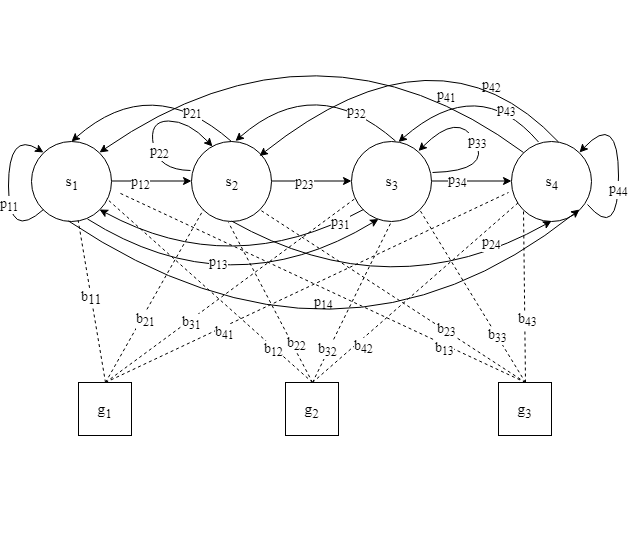
\includegraphics[width=0.48\textwidth]{ahmm.png}
    \caption{General Representation of an Adjusted Hidden Markov Model. In this figure, states, emissions, and respective transition and emission probabilities are shown}
    \label{fig:hmm}
\end{figure}

The specific environment we are studying involves multiple lanes with multiple vehicles that can change their velocities and their lanes. Within this environment, we are able to set up two AHMMs to capture the behaviors we expect to see. The AHMMs are applied to all of the agents, $q$ in our sensing range $R$.

The two AHMMs will aim to predict future velocities $v$ and lanes $l$ of the agents. In this model,

\begin{equation}
    S_v = \{v_1,\ldots, v_n\}
\end{equation}
\begin{equation}
    S_d = \{d_1,\ldots,d_n\}
\end{equation}

    where $S_v$ is states pertaining to velocity and $S_d$ is a set of states pertaining to following distance between an agent $q$ and a preceding agent. The emissions reflect the actions performed between two consecutive states. For velocity we consider the following 3 emissions,

\begin{enumerate}
    \item Speeding Up, if $v(t) > v(t-1)$
    \item Slowing Down, if $v(t) < v(t-1)$
    \item Maintaining Speed, if $v(t) \approx v(t-1)$
\end{enumerate}
%\NB{if not where}

For the lanes,  the distances in $S_d$ are used to identify when lanes change: $l(t) \neq l(t-1)$. The lanes themselves are modeled as states as well:

\begin{equation}
    S_l = \{l_1,\ldots,l_n\}    
\end{equation}

The following 3 emissions are considered:

\begin{enumerate}
    \item Changing Left
    \item Changing Right
    \item Not Changing
\end{enumerate}


\section{AHMM-Based Online Prediction and Model Updates} \label{sec:ahmmpredupdate} %\NB{perhaps combine with next and add Update in the title}
  Using the HMM approach outlined in Section \ref{sec:fmwk}, given enough observations, we can extract a model for each surrounding vehicle. This model can be used online to predict future states of the system, and this is achieved by collecting more observations online. These online observed states can then be applied to the available emission and transition matrices, as lookup tables, to obtain the most likely future state. The future state is determined using:
 %\NB{Using the HMM approach outlined in Section...given enough observations, we can extract a model for surround vehicles}. \NB{This model can be used online to predict future states of the system. This is achieved by collecting more observations online. The observed states at time t can then be used in the available emission and transition matrices, as a lookup table, to obtain the most likely next state}At $t$, the parameters of the AHMM can be used to make online predictions about the future states of the observed system. This is done by identifying the current state, $s_{i}(t)$ and applying it to the transition and emission matrices, which are used as lookup tables, to obtain the next most likely state and its likelihood. %We start with the assumption that $\mathcal{P}$ will give conclusive results from which we can predict the future state as follows\NB{remove this}:
%\begin{equation} \label{eq:nextstate}
%    s_{i}(t+1) = \max_{j}[\mathcal{P}_{i(t),j}]
%\end{equation}
%\NB{this equation is wrong. a state is not equal to the probability!}
%There is, however, the possibility that there will be more than one returned states, as the maximum transition probability %can be the same for multiple states. In this situation, we invoke the use of $\mathcal{B}$:
%\begin{equation} \label{eq:nextemis}
%    g_{k}(t+1) = \max_{k}[\mathcal{B}_{i(t),k}]
%\end{equation}
%\NB{this should be only between the two that are uncertain and that formula is not resolving the issue! }
%\NB{equation needed}.

\begin{align} \label{eq:pred}
   s(t+1) &= s_j \vert \{s_j = \argmax_s \mathcal{P}(s(t)\to s_j) \text{ \& } \nonumber \\ 
   & g(s(t)\to s_j) = \max_g(s(t)\to g_k)\}
\end{align}

%Because the relationship between states and observations is not hidden, we can use the expected inference, derived from \eqref{eq:pred} to assess which returned state is more accurate \NB{not clear, rewrite}.

In the event that \eqref{eq:pred} returns more than one state, we choose the more dangerous transition, which depends on the specific application. For instance, in our case, the more dangerous transition is one that minimizes the distance between our user's vehicle and the observed vehicle.
%\NB{go to another line}

Using this approach, we can predict a series of future states over any horizon $H$ by assuming that each prediction for $t+1$ is correct. We re-use the emission and transition matrices to predict next state at $t+2$ and so on, up to horizon $H$. It is, however, important to note that as $H$ is increased, every successive prediction tends to be less accurate, as the sequence of future predictions is built assuming each of the previous predictions is correct.
%\NB{flip the order} \NB{explain the algorithm}.
Algorithm \ref{alg:pred} shows how we carry forward this prediction through $H$.%\NB{fix this sentence}.
In this algorithm, an observed state, $s(t) = s_i$, is used in %\NB{in not with} 
$\mathcal P$ and $\mathcal B$ to find the most likely next state, $s(t+1) = s_{j^*}$ %\NB{$s_j^*$}.
The following state, $s(t+2)$ is calculated using the previously determined $s_{j^*}$, assuming that it is the next observation. This process is repeated up to $t+H$, such that we have an series $\{s(t+1),\ldots,s(t+H)\}$.
%\NB{assuming that next observation is be the predicted $s(t+1)$}. This process is repeated up to $t+H$.

\begin{algorithm}[ht!]
\caption{Future State Prediction} \label{alg:pred}
\begin{algorithmic}[1]
\WHILE{$t\leq t+H$}
\STATE $t \gets t+1$
\FOR{$s(t) = s_i$}
\STATE $j* \gets \max_j(\mathcal{P}_{i}*)$
\ENDFOR
%\IF{$j$ is not a singleton}
%\FORALL{$j$}
%\STATE{$k \gets j-i$}
%\ELSE
\STATE $s(t+1) \gets s_{j*}$
%\ENDFOR
%\ENDIF
\ENDWHILE
\end{algorithmic}
\end{algorithm}

As previously discussed, a series of prediction becomes less accurate as $H$ increases. In order to alleviate this issue, we propose a method to update $\mathcal{P}$ and $\mathcal{B}$ online. This is achieved by using \eqref{eq:transbuild} and \eqref{eq:obsbuild}, where we adjust $N_{ij}$ and $N_{ik}$, and therefore, $p_{ij}$ and $b_{ij}$ will change. As a result, new parameters $\mathcal{P'}$ and $\mathcal{B'}$ are created to reflect the updates. In addition, we use a sliding window approach such that the size of the training set is always a constant $T$. %\NB{is always constant $T$}\NB{remove this last part}.
The training set is kept the same size in order to retain computational efficiency and to avoid keeping older and less reliable data. Another option would be to discount older data, however we decide not to use this method in this paper because the transition and emission matrices will grow larger, decreasing the efficiency of the proposed method. %\NB{simplify}
$\mathcal{P'}$ and $\mathcal{B'}$ are updated each iteration and will continue to be used for online prediction, making each prediction up-to-date with the online observations.  %\NB{rewrite}

\section{Online Model Fitting}\label{sec:omf}
Using the framework described in Sections \ref{sec:fmwk} and \ref{sec:ahmmpredupdate}, we can extract a model that captures the behavior of a system that we have been observing for $T$. Multiple models can be extracted using several data sets, and with that we can obtain super-sets containing all the transition and emission matrices for multiple vehicles. It is important to note that these models capture different behavioral tendencies, and we assume that we have enough different models to fit any new system during run-time. $\mathcal{M} = \{M_1,\ldots,M_m\}$ is the set of all models, where $m$ indicates the total number of models. The transition and emission matrices of these models are denoted as follows: %\RP{reorder later} %\NB{here we should probably remind the reader that these models capture different behaviors and we assume that we have enough behaviors to model any system during run-time. This concept should be clear also in the introduction}: 
\begin{equation}
    \hat{\mathcal{P}} = \{\mathcal{P}_1,\ldots,\mathcal{P}_m\}
\end{equation}
\begin{equation}
    \hat{\mathcal{B}} = \{\mathcal{B}_1,\ldots,\mathcal{B}_{m}\}
\end{equation}

%\NB{where $M\in\mathbb{N}$ represents the number of models}.

During run-time we observe new measurements of other vehicles. The challenge here becomes fitting each vehicle's observations to the right model computer offline. However, until we have enough observations, the prediction may not be accurate. Thus, we need to take into account possible errors in the prediction, $e$ as we are matching the vehicle behavior with the offline models. 

%In efforts to minimize situations where transitions are unclear, we propose training multiple models prior to the prediction process.\NB{??? What does this last sentence mean?} \NB{just say that we assume to have collected enough models offline to be able to fit and match any new vehicles that appear in our range}

%\NB{We treat any vehicle observed online as a new system and follow the approach outlined in Section...to obtain P and B. At each iteration P and B are updated and compared with the existing Models. The closest model is chosen to predict the behavior of the system. }Having built multiple models, we observe a new vehicle and begin to execute the framework discussed in Section \ref{sec:fmwk} for two consecutive measurements, $\left[o(t-1),o(t)\right]$. With this information, we are able to further execute the framework and determine parameters $\tilde{\mathcal{P}}$ and $\tilde{\mathcal{B}}$, which stand for the transition and emission matrices for the system we are currently observing. In order to determine the optimal model, we calculate the set of errors, $\hat{e}_{N_{M}} = \{e_{N_1},\ldots,e_{N_M}$\} between our model and each of the offline models:

We treat any vehicle observed online as a new system and follow the approach outlined in Section \ref{sec:fmwk} to obtain $\tilde{\mathcal{P}}$ and $\tilde{\mathcal{B}}$. At each iteration, these matrices are updated using the method discussed in \ref{sec:ahmmpredupdate}, and are compared with those of the existing models, $\hat{\mathcal{P}}$ and $\hat{\mathcal{B}}$. The closest model is chosen to predict the behavior of the system. In order to do this, we calculate the error between each model and our current transition and emission matrices:

\begin{equation}
    \forall{P_i} \in \hat{\mathcal{P}}: \hat{e} = \lVert\tilde{\mathcal{P}}-\hat{\mathcal{P}}_{i}\rVert_{l1/l2}
\end{equation}

where $\hat{e} = \{e_i,\ldots,e_m\}$, and $i\in\mathbb{N}^m$

%\NB{revise this}
In order to determine the model with the lowest error, we find the model that minimizes $\hat{e}$,

\begin{equation}
    i^* = \argmin_{i}(\hat{e}_{i})
\end{equation}
%\NB{need to check variables here}
%\NB{add argmin}

where $i^*$ represents the model with the least error, or the optimal model. In order to make predictions using the optimal model, we refer to the parameters, $\mathcal{P}_{i^*}$ and $\mathcal{B}_{i^*}$. The procedure to predict future states is shown in Algorithm~\ref{alg:pred}.


%\NB{merge with previous and change to explain better how new data are going to improve your model...}
%If the observed system, however, does not result in an $i^*$ with a low error, the model is updated using the method discussed in Section \ref{sec:ahmmpredupdate} \NB{what does it mean....very confusing}. Because we are attempting to fit the model, rather than build a new one, we have the advantage of having the baseline, the current $N_M^*$ \NB{what is this baseline?}. We are able to leverage the parameters of this model, by  updating $\mathcal{P}_{N_M^*}$ and $\mathcal{B}_{N_M^*}$ as we observe new transitions or make new inferences, much like how we obtain $\mathcal{P}'$ and $\mathcal{B}'$ in Section \ref{sec:ahmmpredupdate} \NB{again very confusing}. In this case, we obtain $\mathcal{P}'_{N_M^*}$ and $\mathcal{B}'_{N_M^*}$. These models can be used to make future predictions using Algorithm \ref{alg:pred}.\NB{this last part is really bad written}


\section{Assistive Control} \label{sec:adapt}


\subsection{Reachability Analysis}

In order to assess risk of collision we need to predict:
\begin{enumerate}[i.]
\item future states of the surrounding vehicles which are obtained by following the procedure outlined in Section \ref{sec:ahmmpredupdate} and
\item the reachable states of $h$ over the horizon $H$.
\end{enumerate}
In some of our current work, we are using Hamilton-Jacobi reachability analysis to predict future states of a system under uncertainties \cite{esen}. In this paper, we consider a simplified approach for reachability in which we assume that:
\begin{enumerate}[i.]
\item The vehicle can move to the adjacent lane in one time step $\delta t$ \label{ass:i}
\item future variations of velocity are bounded $v_h-\delta_v \leq v_h\leq v_h+\delta_v$, with $\delta_v>0$ \label{ass:ii}
\end{enumerate}
Assumption \ref{ass:i} is made in order to treat the situation as a worst case scenario, and assumption \ref{ass:ii} is made to reflect a physical limitation of vehicles.
Three reachable sets are computed assuming:
\begin{enumerate}
    \item $v_h(t+i)=v_h(t)$
    \item $v_{h,\min}(t+i)=v_h(t)-\delta_v$
    \item $v_{h,\max}(t+i)=v_h(t)+\delta_v$
\end{enumerate} with $i=\{1,...,H\}$. Future reachable positions can be easily computed as $x_h(t+i)=v_h(t+i)*\delta t$ for each of the three aforementioned scenarios.  

[Here let's show 3 figures, with the predictions]

Three reachable sets are obtained at each iteration that contains the possible states reached by $h$ assuming different velocities. For example if $h$ is on a 3 lane road and the prediction horizon is 3 time steps, assuming three velocity case above, then we obtain a total of 45 predictions (15 predictions for every velocity and 3 predictions for every time step, one for each lane/time), as shown in Fig. \ref{fig:reach}.
\RP{dont forget to add picture}
\RP{Predicting for H allows for trajectory generation for motion planning applications as well}

\subsection{Risk Assessment}

 In this section, we discuss how the AHMM method is used to guarantee safety for a HAV, $h$ over a time horizon $H$. 
 
 %\NB{which vehicle? Any?}. In this situation \NB{what situation?}, we have our manned vehicle, $h$, and we have all of the vehicles in our vehicle's sensing range, $R_h$ \NB{$N_{R_h}$ vehicles are in range and can be monitored by $h$ \NB{remember to acknowledge that some vehicles may intermittently enter and exit the range of h}}:
 
 Risk is determined by computing the relative distance between $h$ and all vehicles $q\in R_h$ over the predictive horizon $H$. It is important to note that some vehicles may intermittently enter and exit the range $R_h$, and $q\in\mathbb{N}^n$
where $n$ is the total number of vehicles in the sensing range.

%These vehicles will be referred to as agents in the rest of this work \NB{why??? What's wrong with vehicles? Please remove}.

By using the prediction approach presented in Section \ref{sec:ahmmpredupdate} we can predict future states for all $q$ over an finite horizon $H$ to obtain:

%\RP{Change to bar or tilde or hat for predictions}
\begin{equation}
    \tilde{v}_q = \{v_q(t+1),\ldots,v_q(t+H)\}
\end{equation}

\begin{equation}
    \tilde{l}_q^p = \{l_q(t+1),\ldots,l_q(t+h)\}
\end{equation}

%\RP{put in text}

where $\tilde{v}_q\in S_v$ and $\tilde{l}_q\in S_l$ are the predicted future velocities and lanes for each vehicle $q$, respectively.
With the future velocities, we are able to calculate the forward positions for the horizon $H$ using:
\begin{equation} \label{eq:dumpos}
    \forall{t}\in H: x_q(t) = v_q(t)\delta_t
\end{equation}
where $v_q\in v_q^p$ and $\delta$ refers to a sampling time. With this we obtain future forward positions:
\begin{equation}
    x_q^p = \{x_q(t+1),\ldots,x_q(t+H)\}
\end{equation}
Using this information, we are able calculate relative distance,
\begin{equation}
    \forall q \in R_h: d_q(t) = \lVert x_h(t)-x_q(t)\rVert
\end{equation}

%Generating and using the optimal model for each vehicle $q$, as discussed in Section \ref{sec:omf}, we are able to predict where an agent will be in the environment for the user-defined time horizon, $H$, as discussed in Section \ref{sec:ahmmpredupdate}\NB{this sentence is confusing: By using the prediction approach presented in Section...we can predict future states for $q$ over an finite horizon $H$. }. This time horizon defines how far ahead the user wants the system to check, in order to intervene \NB{remove}. A sequence of future states for agent $q$, both in terms of velocity and lateral position, are developed for $H$ using the AHMM parameters and Algorithm \ref{alg:pred} \NB{merge this with the previous section}. Given a sequence of future predicted velocities,


%In this case, we also assume that the driver will continue the behavior he/she is doing at $t$ up to $t+H$. With this assumption, we are able to the estimate the future positions of $h$, obtaining the set:
%\begin{equation}
%    x_h^p = \{x_h(t+1),\ldots,x_h(t+H)\}
%\end{equation}

%\RP{Simplify - Risk is a function of D as follows}
Risk is a function of $d_q(t)$ such that risk increases as distance decreases and is calculated as follows:

\begin{equation}
    r_{q}^{l}(t) =
    \begin{cases}
    \frac{1}{d_{q}(t)},  & \text{if } l_h=l_q \text{ and } d_{q}(t) > 1  \\
    \frac{1}{\xi d_{q}(t)},  & \text{if } l_h\neq l_q \text{ and } d_{q}(t) > 1  \\
        1,                     & \text{otherwise}  
    \end{cases}
\end{equation}

where $\xi$ is a function of the lane separation, and $r_{q}^{l}(t)$ represents the risk associated with vehicle $q$, evaluated at lane $l$ at time $t$.

%The set of all risks for each vehicle will be denoted as $\mathcal{R}_q$, where
%\NB{what you mean interfering?}

%\begin{equation}
%    \forall{q} \in R: \mathcal{R}_q =
%                    \begin{bmatrix}
%                        r_q^l(t+1) & \dots & r_q^l(t+1) \\
%                        \vdots & \ddots & \\
%                        r_q^l(t+H) &    & r_q^l(t+H)
%                    \end{bmatrix}
%\end{equation}
%\NB{rewrite mathematically this}
It is important to note that multiple vehicles affect risk in our analysis, and the areas with the highest risk are considered for adaptation. The set of maximum risk values in each lane with each velocity for all other vehicles is evaluated as follows: %\RP{Address that to velocities}
\begin{equation}
    \forall q\in R_h,\forall{l}\in{S_l}: r_{q}^l = \max\{r^l_{1},\ldots,r^l_{q}\}
\end{equation}
%\NB{what's L? Define every variable, vector, set, etc...be careful that you may have already defined this before in another way}
Using this, we obtain a distribution of all of the highest risk values for each velocity.

%\begin{equation}
%    \hat{\mathcal{R}} = \{\hat{r}^{L},\hat{r}^{C},\hat{r}^{R}\}
%\end{equation}
%\NB{this doesn't say too much. We can remove it probably}

\subsection{Adaptive User Assistance}

Given the risk distribution, we can assist our user's potentially unsafe actions to guarantee safety. In order to adapt, we need to first identify whether these actions are going to result in a dangerous situation. A user-set range, $[r_\min,r_\max]$ is used as a threshold for risk. Given these values, our system intervenes as follows:
\begin{equation}
    u = \begin{cases}
    u_h & \text{ if } r\leq r_\min \\
    (1-r)u_h + r u_a & \text { if } r_\min<r<r_\max \\
    u_a & \text{ if } r\geq r_\max
    \end{cases}
\end{equation}

where $u_a$ and $u_h$ represent autonomous and human inputs, and $u$ represents the input to the vehicle $h$. In the case that the autonomous control input surpasses that of the user input, the system analyzes the correct action to take. Because the risk is calculated for each lane, the initial action is to identify if a certain lane has a lower risk. With this, we identify $l^*$, which is the lane with the lowest risk:

\begin{equation}
    l^* = \min_l(\mathcal{\hat{R}})
\end{equation}

In addition, we consider the fact that a lane change may be unavailable or unfeasible due to environmental constraints. In this case, we determine the minimum and maximum velocities our vehicle should be driving within one lane. In order to calculate these values, we first find a range $[d_{\min},d_{\max}]$ that our vehicle must be within, in order to ensure that the risk stays below $\rho$. After these safe distances are determined, a maximum velocity and minimum velocity are found such that this range is not violated for horizon $H$.

\RP{1. if one of the vs is safe, then we do that}

\begin{equation}
    v_{\min} = d_{\min}/H
\end{equation}

\begin{equation}
    v_{\max} = d_{\max}/H
\end{equation}

% Let us take, for example, our host vehicle travelling at a much higher velocity than a preceding agent in the same lane. Our system identifies that our user has not shown any sign of turning, and because of that, we assume the user's priority is to stay in the lane. As a result of this, the $u_a$ involves lowering the velocity first. Assuming that the user doesn't respond, our system will continue to lower the velocity such that $u_s = v_q$, as long as the risk remains below $\rho$. If the user responds with a sub-optimal lane change, then the system will assist the user by reverting to the optimal action instead.  


\section{Simulations} \label{sec:sims}
The simulations for this work primarily were done in Matlab. Different simulations were run for each part of the approach shown above. We first discuss how the models were trained, and we validate those results for both velocity and lateral positions. This is followed by showing an example of fitting one model given multiple pre-trained models and a new system to observe. Lastly we demonstrate the risk estimates, and the adjustments made to user actions, in order to verify that we are able to guarantee safety.

\subsection{Training Models}
For training the models, we used a workspace featuring $15$ stationary obstacles. A test vehicle drove through a highway setting with these obstacles, and it was observed for a training period of 700 iterations. This is followed by an estimation period of 700 iterations, which were used to validate the parameters.

\begin{figure}[ht]
    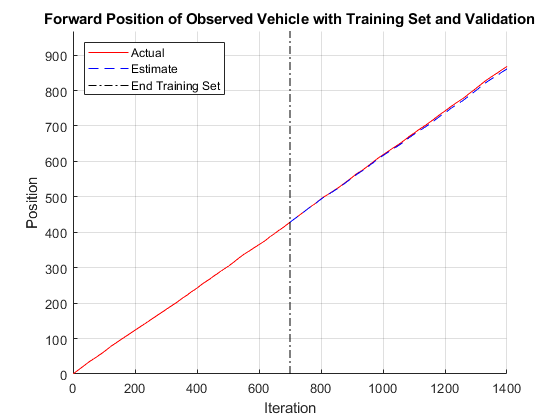
\includegraphics[width=0.48\textwidth]{train1.png}
    \caption{The forward position of the actual robot (red) is shown. After the training set, a prediction is made and the forward position of the estimate is shown (blue dashed).}
    \label{fig:train1}
\end{figure}

\begin{figure}[ht]
    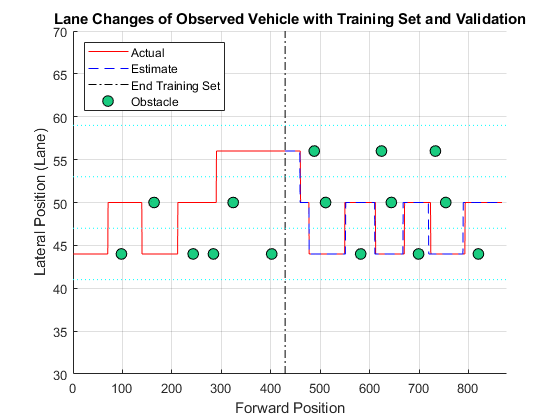
\includegraphics[width=0.48\textwidth]{train2.png}
    \caption{The lane changes of the actual robot (red) are shown. After the training set, a prediction is made and the lateral positions/lane changes of the estimate is shown (blue dashed).}
    \label{fig:train2}
\end{figure}

In this simulation we find that the root mean squared error (RMSE) between the forward positions is $3.9273$, and the RMSE between lane changes is $2.5912$.  

\subsection{Fitting Models}

In the next simulation, we show that we are able to fit pre-trained models to a certain vehicle, whose behaviors are randomly generated, moving through the same workspace as the training sets. In this simulation, we begun to fit the parameters after making one full transition and obtaining related emissions. 

\begin{figure}[ht]
    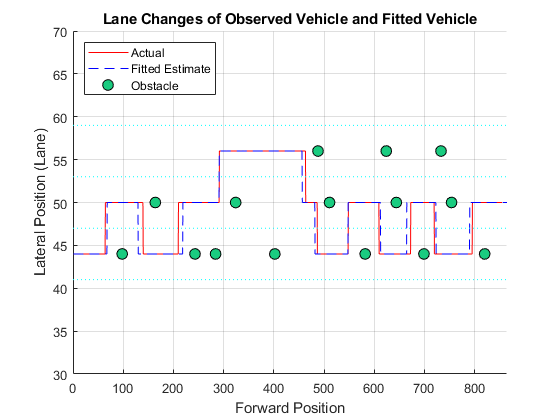
\includegraphics[width=0.48\textwidth]{fit2.png}
    \caption{The forward position of the actual robot (red) is shown. In addition, the forward position of the best-fit is shown (blue dashed).}
    \label{fig:fwd}
\end{figure}

\begin{figure}[ht]
    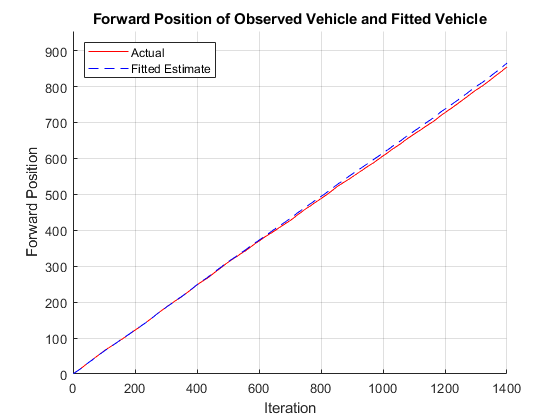
\includegraphics[width=0.48\textwidth]{fit1.png}
    \caption{The lane changes of the actual robot (red) are shown. The lane change predictions of the best-fit are shown (blue dashed).}
    \label{fig:lanchan}
\end{figure}
 In addition, we show the error of the fit for each velocity model in \ref{fig:error}, where we see that the closest fit is that of the medium-speed model.
 
 \begin{figure}[ht]
    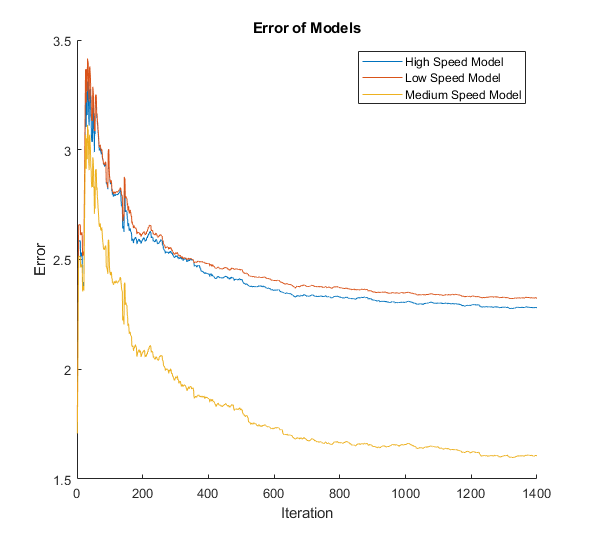
\includegraphics[width=0.48\textwidth]{fit3.png}
    \caption{The error of the fit between our model and each of the three pretrained models}
    \label{fig:error}
\end{figure}
 
 
\subsection{Avoidance}
In order to show the proactive safety system, we have three specific use-cases.

In the first case, the host vehicle in the center lane responds to the actions and future position of a vehicle in the left lane, which is passing a stationary obstacle. The two snapshots of the simulation in Fig.\ref{fig:cs1} and Fig.\ref{fig:cs1b} indicate the behaviors that are occurring.

\begin{figure}[ht]
    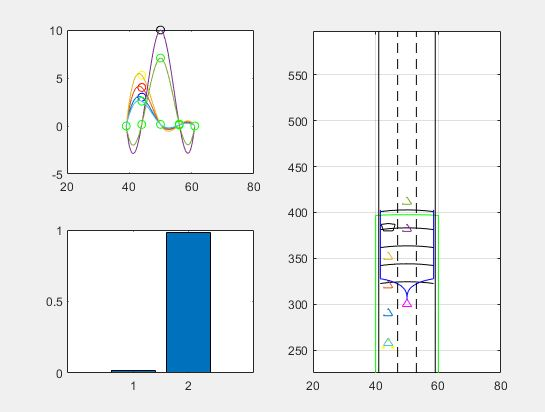
\includegraphics[width=0.48\textwidth]{cs1.JPG}
    \caption{In this snapshot, $u_{\alpha} = 0$ and $u_{h} = 1$. This is because the $r^l$ at $t+H$ is below the $\rho$.}
    \label{fig:cs1}
\end{figure}

\begin{figure}[ht]
    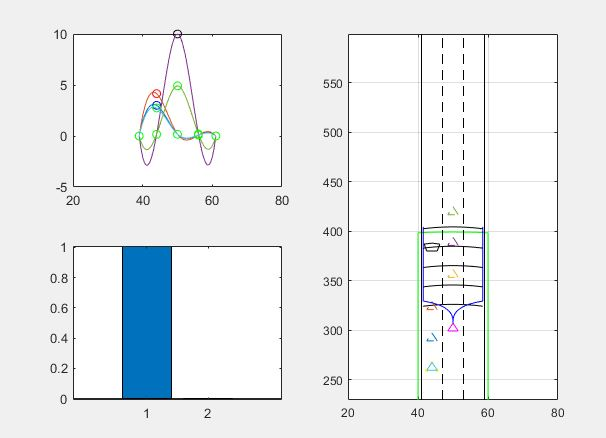
\includegraphics[width=0.48\textwidth]{cs1b.JPG}
    \caption{In this snapshot, the risk in the host vehicle's lane at $t+H$ has increased above $\rho$, and autonomy has increased rapidly. The reason $u_{alpha}$ has increased to 1, is because this is the instant at which the change begins. The location of minimum risk is determined to be the right lane, and the vehicle will then move to the right lane.}
    \label{fig:cs1b}
\end{figure}

This simulation results in a safe operation, as the minimum risk is easily identified and the solution is offered. In this simulation, the human takes no action, which is another reason fully autonomous intervention occurs, and the risk is still minimized and avoided.


In the second simulation, the human does take some action and it is evident that autonomy and human-control are fluid and change based on changing surroundings. In addition, there is once again a clear location at which the risk is at a minimum. The snapshot in Fig.\ref{fig:cs2} shows a situation where the user is travelling at a velocity slightly too rapid for the obstacle ahead, and slowing down will not put it at a risky position in relation to the next vehicle that is behind the user. As a result, $u_{\alpha}$ is increased as the level of risk increases.

\begin{figure}[ht]
    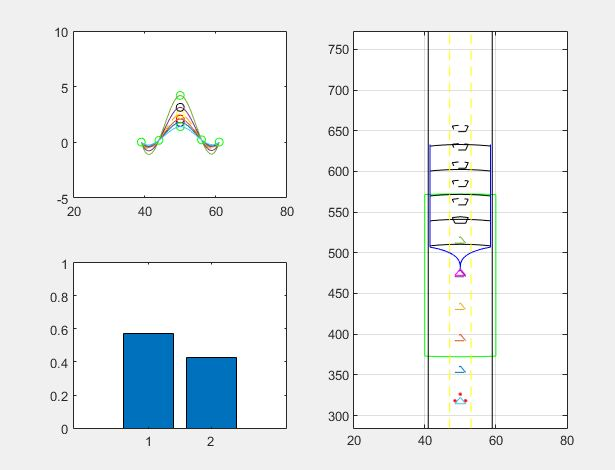
\includegraphics[width=0.48\textwidth]{cs2.JPG}
    \caption{In this snapshot, $u_{\alpha} > u_{h}$. This is because the $r^l_u$ at $t+H$ is above $\rho$}
    \label{fig:cs2}
\end{figure}

This result also indicates a case of the user's desires being met as closely as possible. The user, by only adjusting velocity and not adjusting their lane change behavior, indicates that the velocity is the first parameter to adjust. As shown in Fig.\ref{fig:cs2c}, the velocity is only adjusted so that the driver is in a safe position for the selected time $H$ and, consequently for times $t,t+1,\ldots,t+H$. This is indicated by a velocity that slowly decreases to a safe value. This, however, would only suffice to maximize the time before a collision occurs. Because that is a limitation of only adjusting the velocity, when a collision becomes imminent, $u_\alpha$ increases to 1, and the lane is changed to that of minimum risk.

\begin{figure}[ht]
    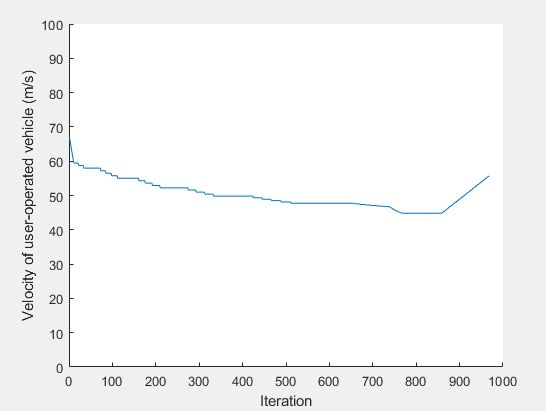
\includegraphics[width=0.48\textwidth]{cs2c.JPG}
    \caption{This figure depicts the velocity of the user's vehicle}
    \label{fig:cs2c}
\end{figure}

The third case is built much like the second case. In this implementation, however, neither of the two surrounding lanes are available. In this case, the system begins to react much like that of the second case, however, there is a error in the prediction of what the following vehicle will do. This is because the model was trained for a lane change, but it is evident that a lane change will not occur when the actual vehicle (not the estimates) approaches our user's vehicle. In a situation like this, the algorithm does delay the imminent collision, but there is a specific preference to retain a certain following distance, $d_q$ behind the obstacle in front. We assume that the user's vehicle has a responsibility to not directly cause a collision on its own. This does, however, leave the possibility of a rear collision, which is addressed further in the discussion.


\section{Conclusions} \label{sec:concs}

\newpage
% references section

% can use a bibliography generated by BibTeX as a .bbl file
% BibTeX documentation can be easily obtained at:
% http://mirror.ctan.org/biblio/bibtex/contrib/doc/
% The IEEEtran BibTeX style support page is at:
% http://www.michaelshell.org/tex/ieeetran/bibtex/
%\bibliographystyle{IEEEtran}
% argument is your BibTeX string definitions and bibliography database(s)
%\bibliography{IEEEabrv,../bib/paper}
%
% <OR> manually copy in the resultant .bbl file
% set second argument of \begin to the number of references
% (used to reserve space for the reference number labels box)

%\begin{thebibliography}{1}

%\bibitem{IEEEhowto:kopka}
%H.~Kopka and P.~W. Daly, \emph{A Guide to \LaTeX}, 3rd~ed.\hskip 1em %plus
%  0.5em minus 0.4em\relax Harlow, England: Addison-Wesley, 1999.
  
  
%\end{thebibliography}

%\printbibliography
\bibliographystyle{abbrv}
\bibliography{mybibliography.bib}


% that's all folks
\end{document}


